\chapter{Simulation}
\label{ch:simulation}

\newthought{\textit{De novo} mutations will undoubtedly take myriad forms} (SNPs, insertions and deletions of varying length, expansions and contractions of short tandem repeats, tandem duplications, non-allelic homologous recombinations, and possibly even inversions).  Detecting all types of variants is a considerable challenge, and the software to do so will be introduced in the next chapter.  In order to measure that software's expected sensitivity and specificity to such variation, we require truth datasets to which we can compare our calls.  A sufficiently small genome (on the order of tens of megabases), could be run on third-generation sequencers, the long reads used to assemble full-length genomes.  Then, the variants called from short-read second-generation sequencing data could be compared to the "truth" dataset established by the newer platform.  This is still very expensive (thousands of dollars for each sample), which limits the number of samples that could be feasibly obtained.  Furthermore, if variants of the classes we are attempting to identify are absent in the handful of genomes we can afford to sequence, we would not be able to accurately ascertain our power.  Finally, it is extraordinarily time-consuming; long-read sequencing experiments require tens of micrograms of genomic, high molecular weight DNA during library construction, which translates to several months of culturing.  For \textit{P. falciparum} parasites which are notorious for being difficult to adapt to culture conditions, this limits the number of samples one can reasonably expect to sequence.

We chose to pursue both a simulation strategy and a validation strategy in order to measure our DNM calling performance.  The results from validation will be presented in Chapter \ref{ch:realdata}.  For the simulation work, we developed two components: first we must generate the genomes of the parents and several children, including each type of DNM we hope to discover.  From these genomes, we must then simulate reads that realistically model errors inherent in our data (matching read lengths, fragment size distributions, single base mismatch errors, indel errors, read pair chimeras, coverage profile, etc.).  We discuss both of these components below.

\section{Simulating genomes}

Simulating a genome merely involves generating an artificial reference sequence in FASTA format.  Our framework is a simple forward simulation of samples.  We first generate the genomes of the parents.  To generate a child's initial genome, we perform recombination \textit{in silico}.  We then add \textit{de novo} mutations on this substrate, thus producing the child's final genome.

We make use of the Variant Call Format (VCF)\cite{Danecek:2011gz}, a text file that encodes one variant per line, specifying the genomic locus, reference and alternate alleles, and metadata for the variant, to describe differences between the two parents and the DNMs to incorporate into the child's genome.  While the \texttt{FastaAlternateReferenceMaker} module in the GATK does purport to generate a new reference sequence based on variants in a VCF, we note that at the time of this writing, it silently fails to incorporate multinucleotide polymorphisms (MNPs) (simultaneous deletion and insertion).  We generate many of these events to remove a reference allele and add an alternate allele in its place (e.g. inversions or gene repertoire replacements).  To include this critical functionality, we developed our own tool to permute an existing reference sequence based on a single-sample VCF file.

Our algorithm, \texttt{IncorporateVariantsIntoGenome}, is described in Algorithm \ref{alg:IncorporateVariantsIntoGenome}.  Briefly, the sequence of each chromosome is loaded into an array, one nucleotide per array element.  We then iterate over each record in the VCF file.  For each SNP or insertion, we replace the reference nucleotide at that position with the entire alternate allele (for insertions, more than a single nucleotide).  For deletions, we replace each corresponding array elements with empty strings.  To generate the new genome, we iterate through each element of the array, emitting the string found in each position.

Note that we chose not to process each variant iteratively as insertions (deletions) would increase (decrease) the size of the array, altering the mapping between the VCF positions and the array positions.  Keeping track of the mapping in spite of the changes is cumbersome.  Instead, out scheme of placing all of the variants on the chromosome array first and then emitting the resulting sequence preserves the mapping.  We will revisit this strategy later on in this chapter when we introduce an algorithm to lift data over from the reference genome coordinates to a simulated genome's coordinates.

Algorithm \ref{alg:IncorporateVariantsIntoGenome} could fail to produce a correct FASTA file in the pathological case that there are multiple overlapping variants called at a single locus.  We are careful to avoid that scenario; we set our simulated variants to be placed no closer than $1000$ bp from one another.

\begin{algorithm}
\caption{Generate an alternative reference sequence based on a VCF file.}
\label{alg:IncorporateVariantsIntoGenome}
\begin{algorithmic}[1]
\Function{IncorporateVariantsIntoGenome}{ref, vcf}
    \ForAll{$\textit{chr} \textrm{ in } \textit{ref}$}
        \State $\textit{vcs} \gets \textit{vcf.getVariants(chr)}$

        \ForAll{$\textit{vc} \textrm{ in } \textit{vcs}$}
            \If{$\textit{vc.getType()} \textrm{ == } \texttt{DEL} \textrm{ || } \textit{vc.getType()} \textrm{ == } \texttt{MNP}$}
                \For{$\textit{pos} \textrm{ in } \textit{vc.getPosition()}:(\textit{vc.getPosition()} + \textit{vc.getReferenceAllele().length())}$}
                    \State $\textit{chr[pos]} = ""$
                \EndFor
            \EndIf

            \State $\textit{chr[vc.getPosition()]} = \textit{vc.getAlternateAllele()}$
        \EndFor

        \State $\textit{write(chr)}$
    \EndFor
\EndFunction
\end{algorithmic}
\end{algorithm}

Many algorithms presented in this chapter rely on empirical distributions to model cross-over rates, read fragment size, indel lengths, and positional errors in reads.  In all cases, we use the inverse transform sampling method for pseudo-random number generation from an arbitrary probability distribution given its cumulative distribution function (CDF)\cite{Devroye:2013gi}.  Simply put, we compute the CDF for an empirical probability distribution, generate a random uniform deviate between $0$ and $1$ for the $x$ value, and interpolate the $y$ value from the CDF.

\subsection{Parents}

\begin{table}[]
\centering
\caption{Assembly statistics on publicly available finished and draft \textit{P. falciparum} references, ordered by scaffold N50 length.  Parental samples are shown in boldface.}
\label{tbl:ref_asm_stats}
\begin{tabular}{@{}llllll@{}}
\toprule
Isolate         & Origin                  & Length (Mb)    & Scaffolds      & Scaffolds N50 (Kb) & \%Q40          \\
\midrule
\textbf{3D7}    & \textbf{Unknown}        & \textbf{23.30} & \textbf{16}    & \textbf{1,690.00}  & \textbf{-}     \\
\textbf{HB3}    & \textbf{Honduras}       & \textbf{24.26} & \textbf{1,189} & \textbf{96.47}     & \textbf{93.17} \\
IGH-CR14        & India                   & 21.74          & 849            & 37.02              & 95.49          \\
\textbf{DD2}    & \textbf{Indochina/Laos} & \textbf{20.88} & \textbf{2,837} & \textbf{19.11}     & \textbf{85.66} \\
RAJ116          & India                   & 14.11          & 1,199          & 13.00              & 89.68          \\
VS/1            & Vietnam                 & 18.89          & 5,856          & 4.42               & 74.79          \\
\textbf{7G8}    & \textbf{Brazil}         & \textbf{14.28} & \textbf{4,843} & \textbf{3.87}      & \textbf{71.00} \\
Senegal\_V34.04 & Senegal                 & 13.24          & 4,329          & 3.76               & 76.22          \\
D10             & PNG                     & 13.38          & 4,471          & 3.71               & 71.80          \\
RO-33           & Ghana                   & 13.71          & 4,991          & 3.47               & 69.91          \\
K1              & Thailand                & 13.29          & 4,772          & 3.42               & 73.30          \\
FCC-2/Hainan    & China                   & 12.96          & 4,956          & 3.30               & 69.39          \\
D6              & Sierra Leone            & 13.22          & 5,011          & 3.23               & 71.62          \\
SL              & El Salvador             & 13.19          & 5,193          & 3.08               & 69.41          \\
PFCLIN          & Ghana                   & 42.19          & 18,711         & 2.99               & -              \\
\bottomrule
\end{tabular}
\end{table}

We began by simulating the genomes of two parents using a workflow depicted in Figure \ref{fig:modrefworkflow}.  For convenience, we simulated samples from the 3D7xHB3 cross.  Choosing the existing reference sequence for the 3D7 sample obviates the need to generate any data for the first parent.  The second parent is tricker; while an existing draft reference sequences does exist for HB3, it is of low quality, assembled into thousands of pieces rather than the simple $14$ autosomes we expect (Table \ref{tbl:ref_asm_stats} shows metrics on every \textit{P. falciparum} sample publicly available).  Using the supercontigs from draft reference sequences is hugely cumbersome for simulating recombination as it is not straightforward to decide which chromosomes in the 3D7 genome and which supercontigs should be processed together.

Instead, we chose to produce a new HB3 reference genome sequence by taking the 3D7 reference and inserting the appropriate modifications using Algorithm \ref{alg:IncorporateVariantsIntoGenome}. These modifications are comprised of two parts: introducing the appropriate variants, and replacing the \textit{var} gene repertoire.

\begin{figure}[h!]
  \centering
    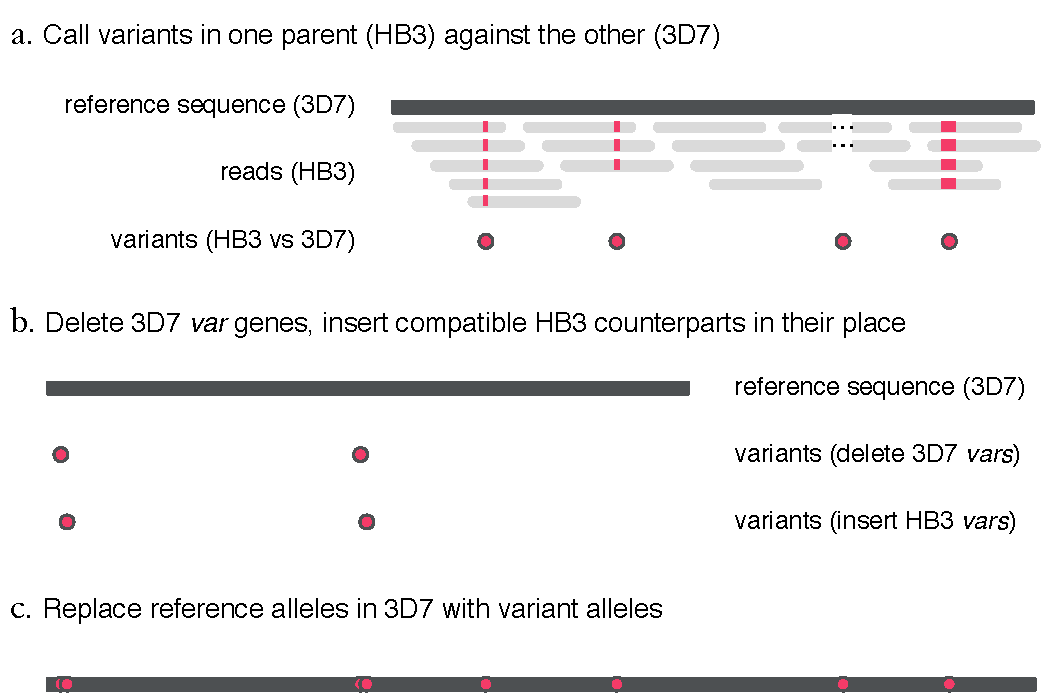
\includegraphics[width=\textwidth]{modrefworkflow}
  \caption{Workflow for generating the HB3 parental genome.  a. Reads from HB3 sample, PG0052-C, are mapped to the 3D7 reference genome, and variants (SNPs and indels) are called and stored as a VCF file.  b. We remove the 3D7 \textit{var} gene repertoire, replacing each with a reasonable HB3 \textit{var} counterpart, and encode the changes to the 3D7 reference genome as a VCF file.  c. We alter the reference genome using Algorithm \ref{alg:IncorporateVariantsIntoGenome}, thus producing the simulated HB3 genome.}
  \label{fig:modrefworkflow}
\end{figure}

We first obtained a VCF of variants found in the HB3 sample, PG0052-C, from the MalariaGen 3D7xHB3 cross dataset\cite{Miles:2015in}.  Variant counts are described in the Table \ref{tb:hb3_variants}, and include SNPs, insertions, deletions, and complex (simultaneous insertions and deletions) events.  These calls were made by combining the results of the reference-based \texttt{UnifiedGenotyper} module in the GATK\cite{DePristo:2011fo} and the reference-free bubble-calling algorithm in the Cortex\cite{Iqbal:2012fx} software.  All calls were restricted to the core genome; subtelomeric regions were masked out due to poor mapping properties (owing to the tremendous diversity in these regions of other \textit{P. falciparum} parasites with respect to the 3D7 reference).

\begin{table}[]
\centering
\caption{Variants found the HB3 (PG0052-C) sample from the MalariaGen 3D7xHB3 dataset.}
\label{tb:hb3_variants}
\begin{tabular}{@{}ccccc@{}}
\toprule
variants & SNPs   & insertions & deletions & complex \\
\midrule
42,054   & 15,376 & 11,807     & 14,643    & 228     \\
\bottomrule
\end{tabular}
\end{table}

Next, we produced a VCF describing \textit{var} gene replacements.  The sequences for HB3 \textit{var} genes and upstream promoter metadata were obtained from the VarDom server\cite{Rask:2010fi}.  No positional information from this data source is available, thus the exact placement of these \textit{var} genes in a chromosomal context is unclear.  However, previous work has established a strong association between conserved sequences of upstream promoters (phylogenetically grouped into five classes: A through E) and placement in the genome\cite{Kraemer:2006gv}.  We therefore replaced 3D7 \textit{var} genes with HB3 \textit{var} gene counterparts, taking care to replace genes with similar UPS classes whenever possible, and grouping genes with suspiciously incomplete metadata otherwise. The replacements were described in the resulting VCF as simultaneous deletions of the 3D7 allele and insertions of the HB3 allele.  No effort was made to match the orientation of the replacement \textit{var} gene with the replaced \textit{var} gene. The precise replacements are summarized in Table \ref{tb:hb3_vars}.

\begin{table}[]
\centering
\caption{\textit{Var} gene replacements from 3D7 to HB3 repertoire.}
\label{tb:hb3_vars}
\begin{tabular}{@{}llll@{}}
\toprule
3D7 gene & 3D7 ups class & HB3 gene & HB3 ups class \\
\midrule
PF3D7\_0421100 & UPSB5 & PFHG\_02500 & UNKNOWN \\
PF3D7\_0600200 & UPSB2 & PFHG\_02495 & UNKNOWN \\
PF3D7\_0632500 & UPSB5 & PFHG\_05132 & UNKNOWN \\
PF3D7\_0800300 & UPSB2 & PFHG\_04012 & ND \\
PF3D7\_1200400 & UPSB5 & PFHG\_05200 & ND \\
PF3D7\_1240900 & U     & PFHG\_05483 & ND \\
PF3D7\_0400400 & UPSA1 & PFHG\_03840 & UPSA1 \\
PF3D7\_0425800 & UPSA1 & PFHG\_03671 & UPSA1 \\
PF3D7\_1100200 & UPSA1 & PFHG\_04861 & UPSA1 \\
PF3D7\_1150400 & UPSA1 & PFHG\_05052 & UPSA1 \\
PF3D7\_1300300 & UPSA1 & PFHG\_03234 & UPSA1 \\
PF3D7\_0533100 & UPSA2 & PFHG\_03521 & UPSA2* \\
PF3D7\_0100300 & UPSA3 & PFHG\_02274 & UPSA3 \\
PF3D7\_0100100 & UPSB1 & PFHG\_04081 & UPSB1 \\
PF3D7\_0115700 & UPSB1 & PFHG\_04749 & UPSB1 \\
PF3D7\_0200100 & UPSB1 & PFHG\_03516 & UPSB1 \\
PF3D7\_0223500 & UPSB1 & PFHG\_04277 & UPSB1 \\
PF3D7\_0300100 & UPSB1 & PFHG\_03717 & UPSB1 \\
PF3D7\_0324900 & UPSB1 & PFHG\_04035 & UPSB1 \\
PF3D7\_0400100 & UPSB1 & PFHG\_04491 & UPSB1 \\
PF3D7\_0426000 & UPSB1 & PFHG\_04620 & UPSB1 \\
PF3D7\_0500100 & UPSB1 & PFHG\_04593 & UPSB1 \\
PF3D7\_0632800 & UPSB1 & PFHG\_04770 & UPSB1 \\
PF3D7\_0700100 & UPSB1 & PFHG\_04057 & UPSB1 \\
PF3D7\_0712300 & UPSB1 & PFHG\_03232 & UPSB1 \\
PF3D7\_0733000 & UPSB1 & PFHG\_04928 & UPSB1 \\
PF3D7\_0800100 & UPSB1 & PFHG\_03416 & UPSB1 \\
PF3D7\_0413100 & UPSB3 & PFHG\_03476 & UPSB3* \\
PF3D7\_0712400 & UPSB3 & PFHG\_02421 & UPSB3 \\
PF3D7\_1240300 & UPSB4 & PFHG\_02272 & UPSB4 \\
PF3D7\_0809100 & UPSB6 & PFHG\_02276 & UPSB6 \\
PF3D7\_0712800 & UPSB7 & PFHG\_04014 & UPSB7 \\
PF3D7\_0808700 & UPSB7 & PFHG\_02425 & UPSB7 \\
PF3D7\_1240400 & UPSB7 & PFHG\_04769 & UPSB7 \\
PF3D7\_0412400 & UPSC1 & PFHG\_03480 & UPSC1 \\
PF3D7\_0412700 & UPSC1 & PFHG\_03478 & UPSC1 \\
PF3D7\_0412900 & UPSC1 & PFHG\_00592 & UPSC1 \\
PF3D7\_0420700 & UPSC1 & PFHG\_02419 & UPSC1 \\
PF3D7\_0420900 & UPSC1 & PFHG\_02429 & UPSC1 \\
PF3D7\_0421300 & UPSC1 & PFHG\_02277 & UPSC1 \\
PF3D7\_0617400 & UPSC1 & PFHG\_02273 & UPSC1 \\
PF3D7\_0712900 & UPSC2 & PFHG\_04015 & UPSC2 \\
PF3D7\_1200600 & UPSE  & PFHG\_05046 & UPSE  \\
\bottomrule
\end{tabular}
\end{table}

These two VCFs were combined to produce a complete set of changes required to transform the 3D7 genome into a pseudo HB3 genome.  The transformation was applied using Algorithm \ref{alg:IncorporateVariantsIntoGenome}.

\section{Children}

Generating the genomes of the children is slightly more involved, as there is much more biology to simulate, and many more considerations to be made when placing variants. We generated VCF descriptions of the children using a multi-stage workflow shown in Figure \ref{fig:generatechildrenpipeline}.  In order, we simulate:

\begin{enumerate}
    \item homologous recombination between 3D7 and HB3 genomes
    \item gene conversion events
    \item NAHR events between compatible \textit{var} genes
    \item \textit{de novo} SNPs, insertions, deletions, and inversions
\end{enumerate}

\begin{figure}[h!]
  \centering
    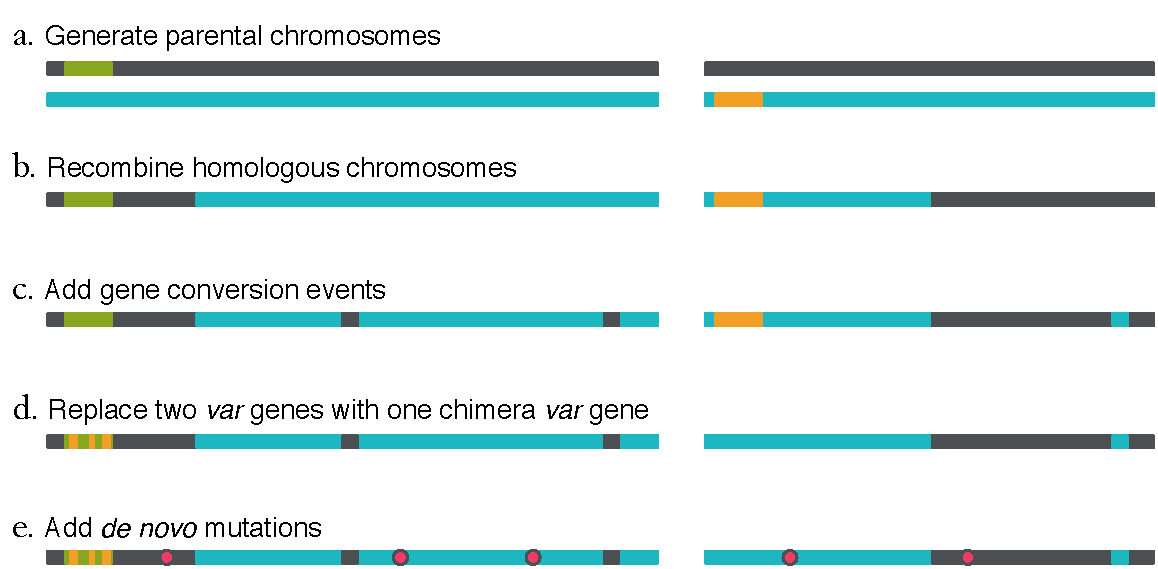
\includegraphics[width=\textwidth]{generatechildrenpipeline}
  \caption{Workflow for generating children's genomes.  a. Generate chromosomes from the parental genomes (compatible \textit{var} genes shown in green and orange).  b. Recombine homologous chromosomes.  c. Add gene conversion events (by incorporating variants from the alternative haplotypic background over a limited genomic window).  d. Replace one of the \textit{var} genes with a chimera of compatible genes.  e. Add \textit{de novo} mutations.}
  \label{fig:generatechildrenpipeline}
\end{figure}

\subsection{Homologous recombination}

\subsubsection{Allelic homologous recombination}

\begin{figure}[h!]
  \centering
    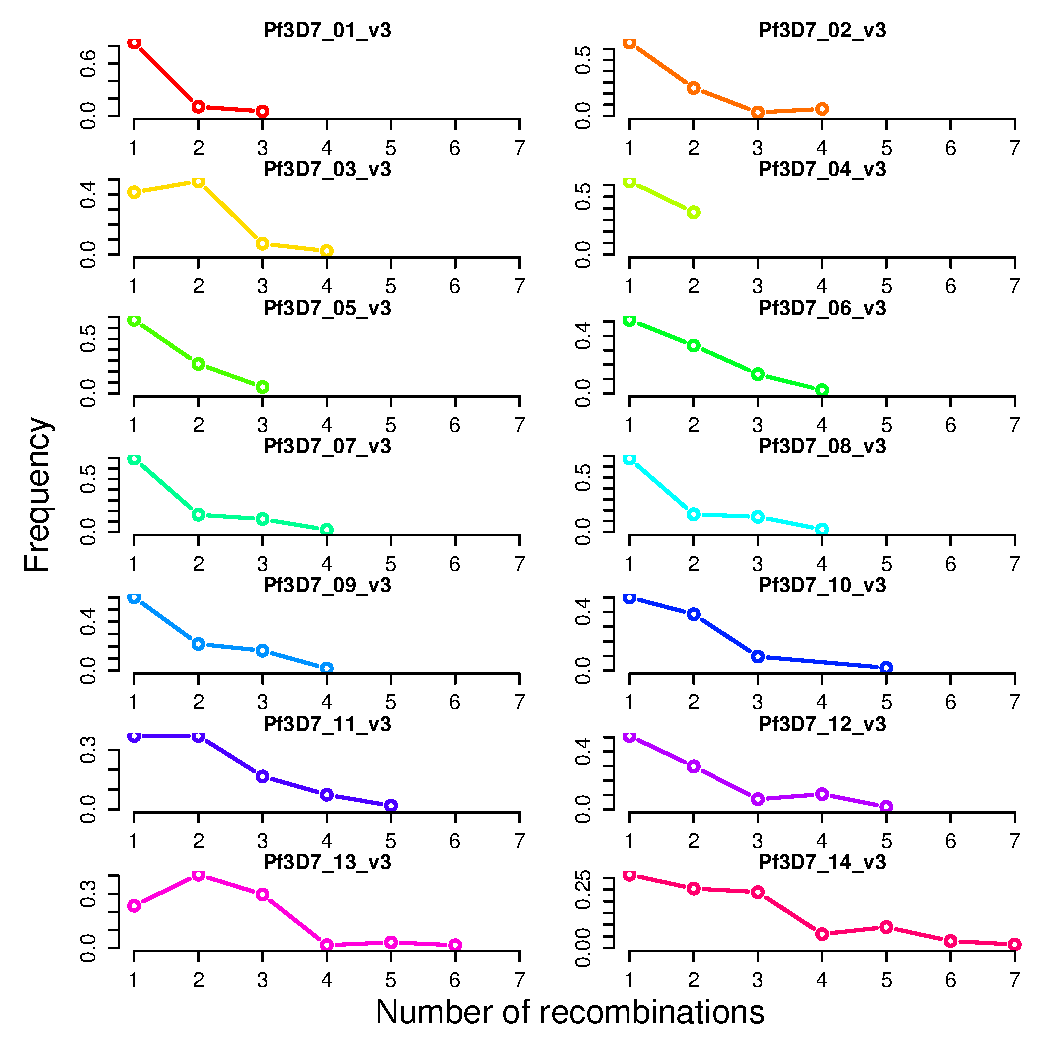
\includegraphics[width=\textwidth]{recomb-1}
  \caption{Empirical recombination frequencies per chromosome}
  \label{fig:recomb-1}
\end{figure}

For each bivalent chromosome, the cross-over rate will be dependent on the length of the chromosome. The empirical distributions for bivalent formation and crossover were generated from the $75$ samples in the MalariaGen crosses data. For each sample, only half of the chromosomes are expected to exhibit cross-over events.  The cross-over rates are plotted in Figure \ref{fig:recomb-1}. We simulated recombination in a sample by first drawing a binary number indicating whether a chromosome should be recombined, and if so, drawing the number of cross-over events per chromosome from these empirical distributions. The recombination sites themselves were chosen by drawing a uniform random variate between $1$ and the length of the chromosome. Although there are certainly hotspots and coldspots of recombination in the genome, we have ignored this complication.  An example haplotype mosaic of chromosome $12$ for five samples is shown in Figure \ref{fig:haplotypes12}.

\begin{figure}[h!]
  \centering
    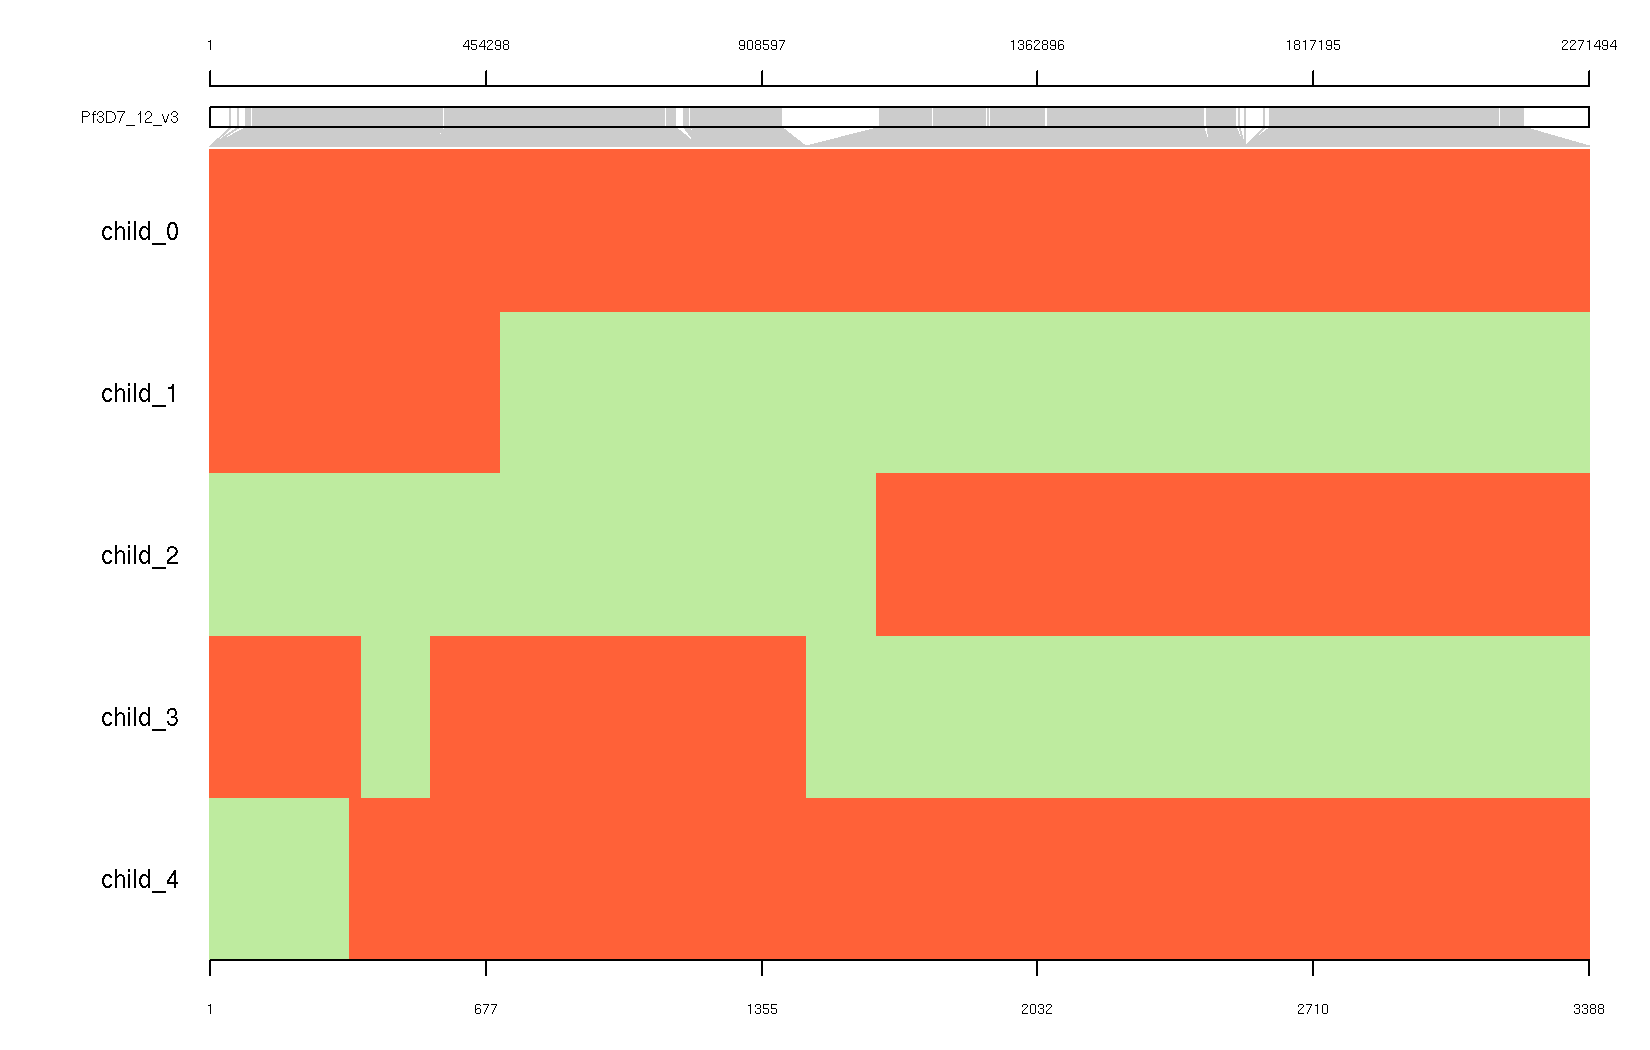
\includegraphics[width=\textwidth]{haplotypes12}
  \caption{Simulated haplotype mosaics for chromosome 12.  Genomic position is shown at the top of the figure, while variant number is shown at the bottom.  Each variant is depicted as a vertical grey line attached to the mosaic plot at the appropriate location.  In the mosaic, every variant is color-coded by parent of origin.}
  \label{fig:haplotypes12}
\end{figure}

\subsubsection{Gene conversion}

To simulate gene conversion events, we first chose a handful of random sites known to be variant in HB3, and determined the size of the event (number of adjacent HB3 variants involved in the gene conversion) by choosing a random uniform variate between $1$ and $3$. If these sites were originally transmitted to the child, they were removed from the VCF. If they had not been transmitted, they were added. The homologous recombinations and gene conversion events are displayed below for each chromosome and sample.

\subsubsection{Non-allelic homologous recombination}

NAHR events were generated by first finding compatible recombination partners. This list was generated by determining which 3D7 \textit{var} genes had been transmitted to the child, grouped by upstream promoter class and telomeric positioning ($5'$ or $3'$). In each group, two random genes were chosen. If necessary, the gene sequences were reverse complemented to have matching orientation (note that the sequences may not have the same orientation in the simulated genomes themselves). As NAHR events between two \textit{var} genes appear to occur in regions of homology, we identified shared $9$-mers, positioned between $20$ bp and $100$ bp between the two genes, to act as possible recombination sites. We randomly selected between $2$ and $5$ of these positions to act as recombination breakpoints, switching between the sequences and copied sequence data accordingly. Keeping in mind that our previous work has shown that the recombined \textit{var} genes are lost in order to produce the chimera, we added VCF records to delete the previous \textit{var} alleles from the child's genome and replace one of them with the recombined sequence.

\begin{figure}[h!]
  \centering
    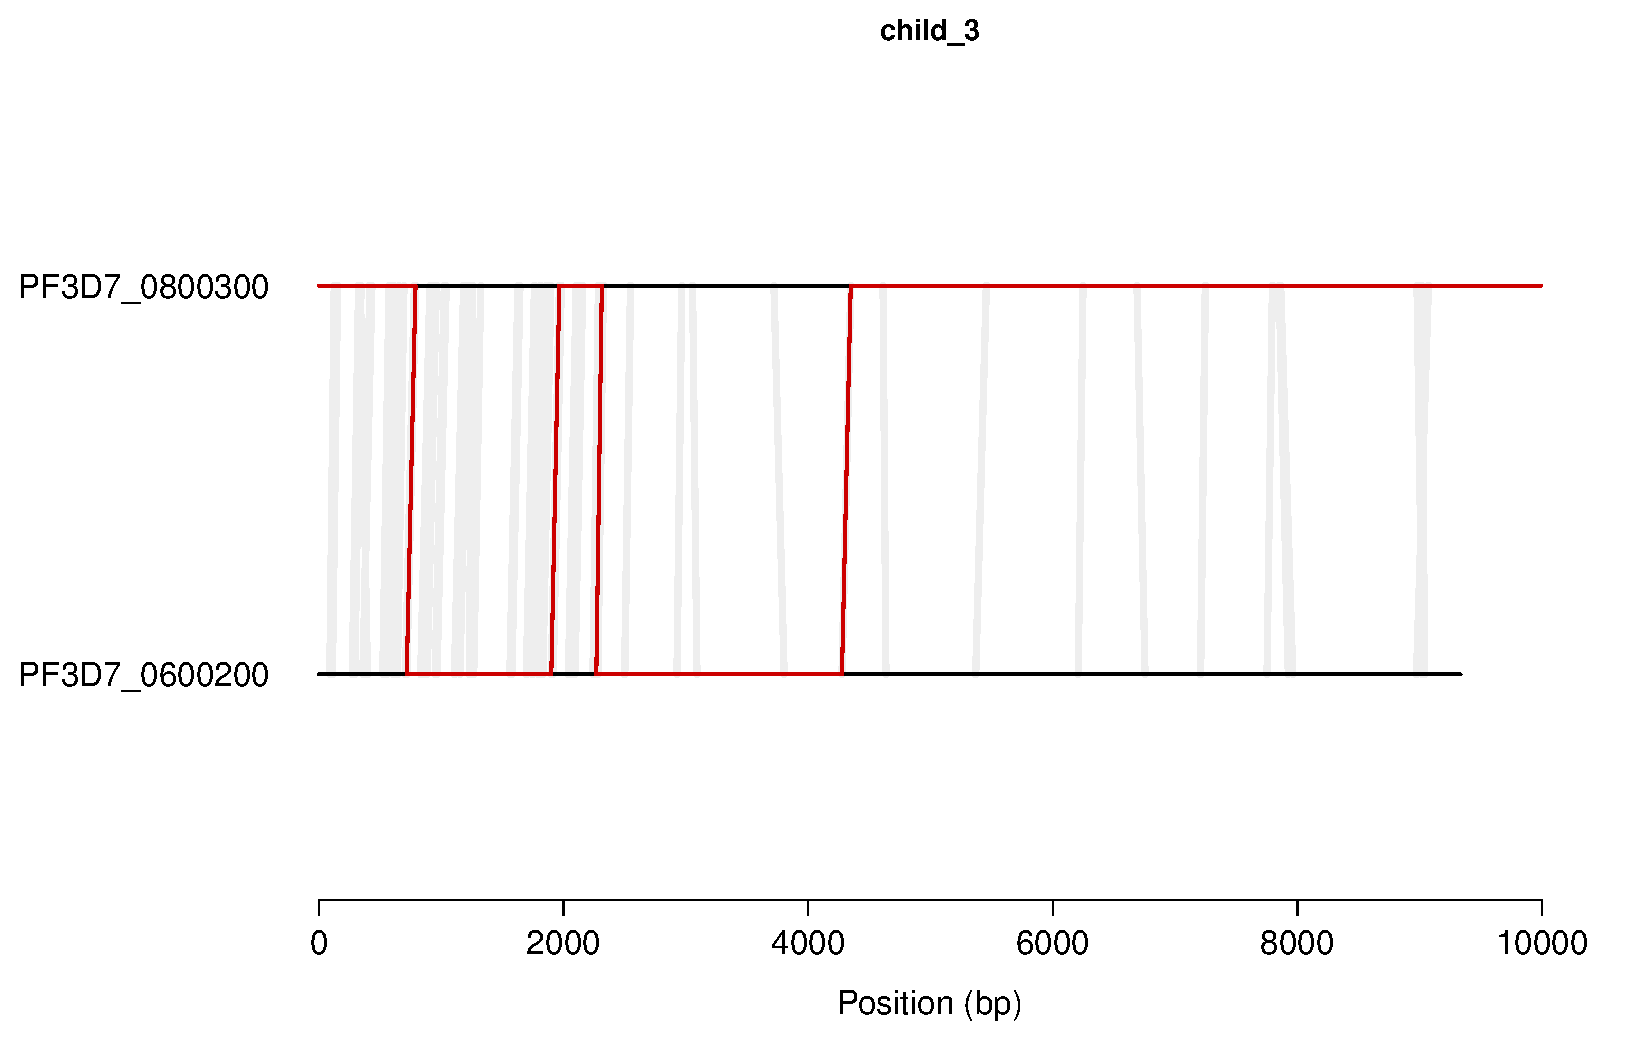
\includegraphics[width=\textwidth]{showrecomb-24}
  \caption{Non-allelic recombinations for two compatible \textit{var} genes.}
  \label{fig:showrecomb-24}
\end{figure}

\subsection{SNPs, insertions, and deletions}

\begin{figure}[h!]
  \centering
    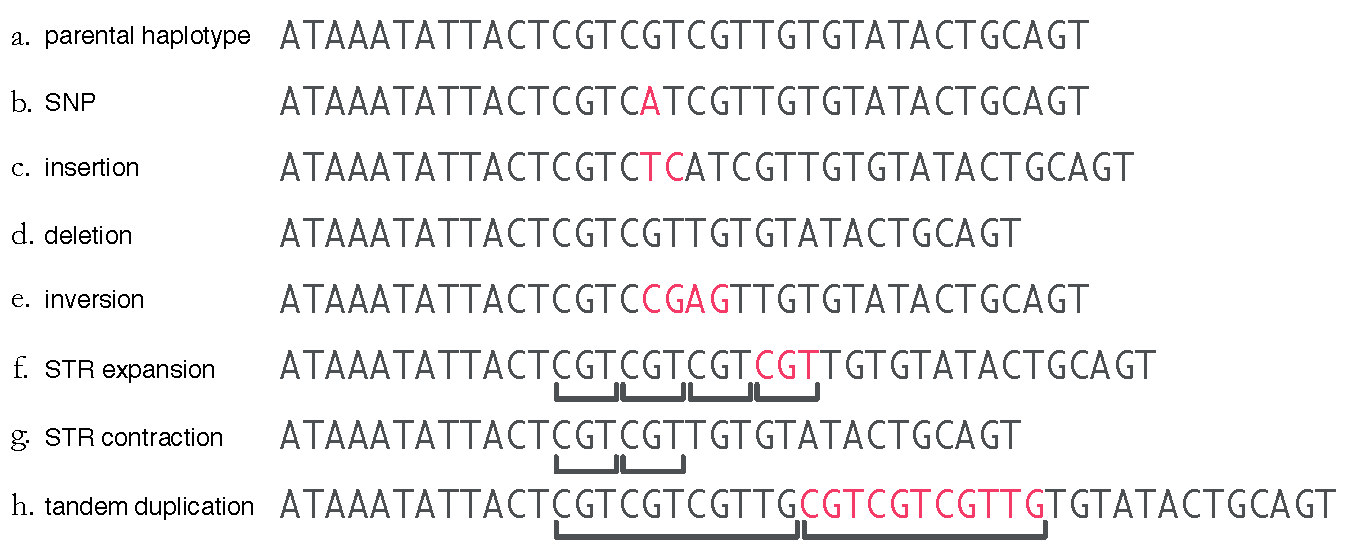
\includegraphics[width=\textwidth]{variants}
  \caption{Simulated variant types.  a. Original, parental haplotypic background upon which variants will be placed.  b. A single nucleotide polymorphism.  c. An insertion of two nucleotides.  d. A deletion of three nucleotides.  e. An inversion of four nucleotides.  f. Expansion of a $3$ bp short tandem repeat (STR) by one unit.  g. A contraction of an STR by one unit.  h. A tandem duplication of $11$ nucleotides.}
  \label{fig:variants}
\end{figure}

With the ground state genome now generated, we further generated simple events - SNPs, insertions, and deletions - on this foundation to complete the production of the child's genome.  The precise number of events can be specified by the user at runtime, and for each simulated genome, different counts were specified.

To simulate \textit{de novo} SNPs, we added sites with random (non-reference) alleles at random positions throughout the genome.  We also simulated insertion, deletion, and inversion events at every length between $1$ and $100$ bp. For insertions, random alleles were generated and tested to ensure they did not match the allele already in the reference sequence. For deletions, we simply replaced the reference allele with a truncated allele of the prescribed length. For inversions, we replace the reference allele with its complement.

\subsubsection{Expansion and contraction of short tandem repeats (STRs)}

As a special case of indels, we sought specifically to simulate the expansion and contraction of short tandem repeats (STRs), depicted in Figure \ref{fig:variants}f-g. STRs are constrained to occur at loci where there are already existing repeats, and expansions (contractions) should manifest as the insertion (deletion) of whole units at a time.  We first built a map of repeated $2$-bp, $3$-bp, $4$-bp, and $5$-bp sequences in the 3D7 genome. We filtered these lists, retaining only STRs where the repeated unit occurred at least three times. For each simulated event, we randomly chose a position from the appropriate list and select a number of units to add or remove. The number of units is constrained to be less than the length of the number of repeat units of the existing STR. With these considerations, we simulated expansions and contractions at the aforementioned repeat unit sizes.

\subsubsection{Tandem duplications}

For tandem duplications (as depicted in Figure \ref{fig:variants}h) of length $l$, we chose positions in the genome at random, copied the next $l$ bases, and inserted an identical copy at the same locus.  Events at each length between $10$ bp and $50$ bp were produced.

\section{Simulating reads}

We now turn our attention to simulating second-generation sequencing reads given an underlying genome.  There are existing tools that will simulate perfect reads and uniform coverage, which will be important for initial tests of our variant identification software.  However, the crucial simulation is of imperfect reads with non-uniform coverage.  Without this, any estimate of our sensitivity and specificity is unlikely to be predictive of performance in real data.

There are many tools that can simulate imperfect reads from a given sequence.  Almost every solution involves user-specified parameters controlling the properties of the sequencing data.  For instance, a tool may model fragment size as a normal distribution, requiring the user to specify the requisite shape parameters.  It may also permit the user to specify a desired mismatch rate to simulate the presence of sequencing error.  Some tools have presets that automatically set parameters to those consistent with average behavior for various sequencing platforms.

The problem with all of these tools is an over-reliance on assumed parameters of real data.  Should a fragment size distribution for real data deviate from the typical normal distribution, this will not be captured in the simulated dataset.  Mismatch and indel errors do not happen at any position in the read with equal probability, but rather are biased towards later cycles and certain sequence contexts.  Read coverage is not simply Poisson-distributed, but varies across the length of the genome depending on GC bias, secondary structure, even the particular sequencing chemistry used.  There are currently no tools that are capable of capturing such nuance.

Instead, we chose to learn empirical distributions of major sequencing properties using an exemplar dataset and sample from those distributions directly in order to generate reads.  This frees us from having to make any assumptions about our dataset, easily generalizes to any dataset regardless of when, where, or how it was sequenced.  It's also vastly more realistic than other approaches.

Our approach is detailed below.  Briefly, it consists of three components:

\begin{enumerate}
    \item A "coverage profile": a description of where every fragment and read in the genome should fall and which should contain errors.
    \item A "read profile": a description of where to place errors within a read, including mismatches, insertions, and deletions.
    \item The read simulator: samples from the profiles to generate reads in the new reference sequence.
\end{enumerate}

\subsection{Constructing the coverage profile}

Construction of a coverage profile consists of two sub-problems: providing a complete description of where reads fall on the existing reference sequence, and transferring that information sensibly to the modified reference sequence.  This is depicted in Figure \ref{fig:coverageprofile}.  We address each of these needs with custom tools.

\begin{figure}[h!]
  \centering
    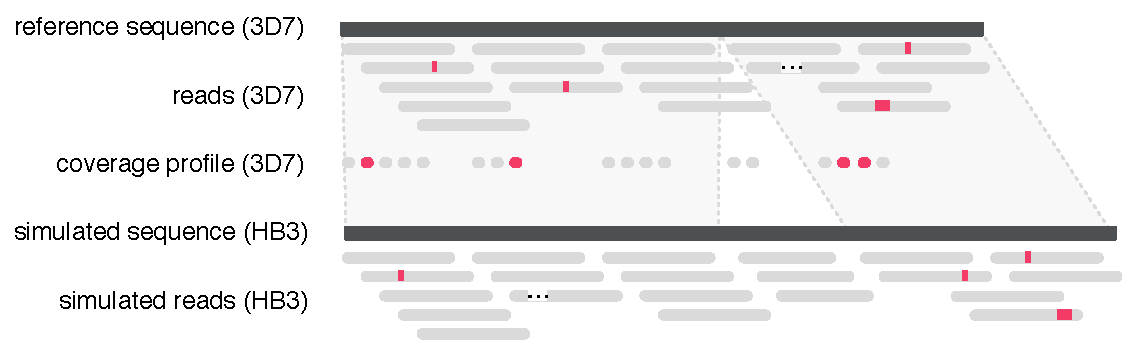
\includegraphics[width=\textwidth]{coverageprofile}
  \caption{Construction of the coverage profile for the reference genome and liftover to the altered genome.  Each read start (and fragment start, not shown) is stored along with a count of the number of reads at that location that contain errors.  This information is then lifted over to the simulated sequence, and gaps in the table are filled in with neighboring values.}
  \label{fig:coverageprofile}
\end{figure}

\subsubsection{Computing read and fragment starts, and error rates}

We developed a tool, \texttt{ComputeBaseAndFragmentErrorRates}, which provides a precise specification for the number of fragments and reads found starting at of every position in the canonical reference genome, as well as an accounting as to which reads and fragments contained any kind of error (mismatch or indels).  Briefly, we iterate over every chromosome in the reference genome, advancing through every aligned read stored in an exemplar sample's coordinate-sorted BAM file.  We instantiate a chromosome-length array indicating the number of reads that start at a given position and the number of reads that contain apparent errors (any discrepancy from the reference sequence).

We must also store information about read fragment starts and error rates, which requires us to keep track of read pairs as we traverse the BAM file.  To do so, we hash the read name to the first instance of the read we see along the length of a chromosome.  As paired-end reads have the same name, the second time we see the same read name, we will have found the second end of the pair.  We then increment the count at the chromosome array position that corresponds to the $5'$-most end of the pair, and increment the fragment errors array based on errors in either end of the pair.

This algorithm is described in Algorithm \ref{alg:ComputeBaseAndFragmentErrorRates}.

\begin{algorithm}
\caption{Emit all fragment starts, read starts, and error rates per position.}
\label{alg:ComputeBaseAndFragmentErrorRates}
\begin{algorithmic}[1]
\Function{ComputeBaseAndFragmentErrorRates}{BAM}
    \ForAll{$\textit{chr} \textrm{ in } \textit{chrs}$}
        \State $\textit{nReadsErrors} \gets []$
        \State $\textit{nReads} \gets []$
        \State $\textit{nFragmentsErrors} \gets []$
        \State $\textit{nFragments} \gets []$
        \State $\textit{seenReads} \gets []$

        \State $\textit{reads} \gets \textit{BAM.getAllReads(chr)}$

        \ForAll{$\textit{read} \textrm{ in } \textit{reads}$}
            \State $\textit{readErrorPositions} \gets \textit{getPositionsErrors(read)}$
            \State $\textit{refErrorPositions} \gets \textit{convertReadPositionsToReferencePositions(readErrorPositions)}$

            \ForAll{$\textit{refErrorPosition} \textrm{ in } \textit{refErrorPositions}$}
                \State $\textit{nReadsErrors[refErrorPosition]}++$
            \EndFor

            \For{$\textit{readPosition} \textrm{ in } 0:\textit{read.length()}$}
                \State $\textit{nReads[convertReadPositionsToReferencePositions(readPosition)]}++$
            \EndFor

            \If{$\textit{!seenReads.contains(read.getName())}$}
                \State $\textit{seenReads} \gets \textit{read.getName()}$
            \Else
                \State $\textit{mateErrorPositions} \gets \textit{getPositionsErrors(seenReads[read.getName()])}$

                \If $\textit{readErrorPositions.size()} + \textit{mateErrorPositions.size()} \ge 1$
                    \State $\textit{nFragmentsErrors[seenReads[read.getName()].getAlignmentStart()}++$  
                \EndIf

                \State $\textit{nFragments[seenReads[read.getName()]}++$  
            \EndIf
        \EndFor

        \For{$\textit{pos} \textrm{ in } 0:\textit{nReads.length()}$}
            \State $\textit{print chr, pos, nReadsErrors[pos], nReads[pos], nFragmentsErrors[pos], nFragments[pos]}$
        \EndFor
    \EndFor
\EndFunction
\end{algorithmic}
\end{algorithm}

\subsubsection{Lifting read profile over from reference to simulated genome}

The genomic coordinates present in the table produced by Algorithm \ref{alg:ComputeBaseAndFragmentErrorRates} must be transformed from the reference sequence to the simulated genome before it can be used.  To do so, we developed a tool that could liftover the coordinates appropriately when given the table, reference sequence, and a VCF file describing the alterations made to the reference to transform it into the simulated genome.  This is accomplished with an algorithm similar to Algorithm \ref{alg:IncorporateVariantsIntoGenome}.  We iterate through each chromosome as we did before, storing the entire sequence as an array of strings, placing alternate alleles in the place of reference alleles, or in the case of deletions, replacing reference alleles with blank strings.  Once the array is populated, we advance through the coverage table one position at a time.  At each position, we emit the contents of the previously constructed table with the number of reads, fragments, and errors for each.  At some positions, insertions will have changed the length of the sequence in the bin, and the extra positions will not have explicit read and fragment information to emit.  To account for this, we keep running statistics on previously seen read and fragment statistics from which we can compute running means and standard deviation.  We generate new values for the number of reads, fragments, and error rates as necessary as the mean plus standard deviation of the relevant metric, ensuring the values are never less than $0$, and that we round up or down to the nearest integer (error rates are rounded up and read/fragment counts are rounded down to increase our self-penalty).

This algorithm is described in \ref{alg:LiftoverFromRefToChild}.

\begin{algorithm}
\caption{Lift a table from reference to child coordinates.}
\label{alg:LiftoverFromRefToChild}
\begin{algorithmic}[1]
\Function{LiftoverFromRefToChild}{ref, vcf, table}
    \ForAll{$\textit{chr} \textrm{ in } \textit{ref}$}
        \State $\textit{newchr} = \textit{IncorporateVariantsIntoGenome(ref, vcf)}$

        \For{$i \textrm{ in } 0:newchr.length()$}
            \State $\textit{emit(table[i])}$
            \If{$newchr[i].length() > 1$}
                \For{$j \textrm{ in } 1:newchr[i].length()$}
                    \State $\textit{emit(extrapolate(table[i]))}$
                \EndFor
            \EndIf
        \EndFor
    \EndFor
\EndFunction
\end{algorithmic}
\end{algorithm}

\subsection{Constructing the read profile}

Next, we generate the read profile, describing the various properties of fragments and read.  As in previous examples, we iterate over each read in the exemplar sample's BAM file, storing relevant information in tabular form.

\subsubsection{Scalar properties}
We first store the following scalar information (as the data we are modelling is assumed to be Illumina data generated from a single library, some properties which could otherwise be stored as distributions are instead treated as a single number that will be simple constants in our simulation):

\begin{enumerate}
    \item read length
    \item number of reads
    \item number of reads with errors
    \item number of read pairs
    \item number of chimeric pairs (each end aligned to different chromosomes)
    \item number of mismatches 
    \item number of insertions
    \item number of deletions
\end{enumerate}

Example values for each of these metrics can be found in Table \ref{tbl:scalarvalues}.  Note that some of the mismatches, insertions, and deletions may represent true variation between the sample and the reference sequence.  We do not mask these sites out.  While this increases the apparent error rate, the variant rates are typically low compared to the number of bases in the reference sequence itself, making the difference negligible.  Furthermore, we will choose the reference sample as the exemplar dataset for the read simulations.  Since this sample should theoretically be identical to the reference sequence, this choice obviates the need for any masking of variants in the reference sample against the reference sequence.

\begin{table}[]
\centering
\caption{Example read and fragment scalar properties for sample PG0063-C.}
\label{tbl:scalarvalues}
\begin{tabular}{@{}lr@{}}
\toprule
                   & PG0051-C\\
\midrule
readLength         & 76\\
numReads           & 38,846,418\\
numReadsWithErrors & 3,696,708\\
numPairs           & 19,473,634\\
numChimericPairs   & 348,294\\
numMismatches      & 6,525,504\\
numInsertions      & 139,941\\
numDeletions       & 317,076\\
\bottomrule
\end{tabular}
\end{table}

\subsubsection{Empirical distributions}

Other properties take on a range of values with some probability.  Rather than trying to fit the underlying distributions explicitly (which can often fail as datasets contain more nuance than what sequencing platforms should theoretically produce), we instead store empirical distributions and generate random values from them accordingly.  We store the following empirical distributions:

\begin{enumerate}
    \item number of errors (of any type - mismatch, insertion, or deletion) in a read
    \item fragment size
    \item insertion size
    \item deletion size
\end{enumerate}

Note that these distributions are not conditioned on position in the read.  Example distributions derived from an exemplar sample are shown in Figure \ref{fig:empDists-1}.

\begin{figure}[h!]
  \centering
    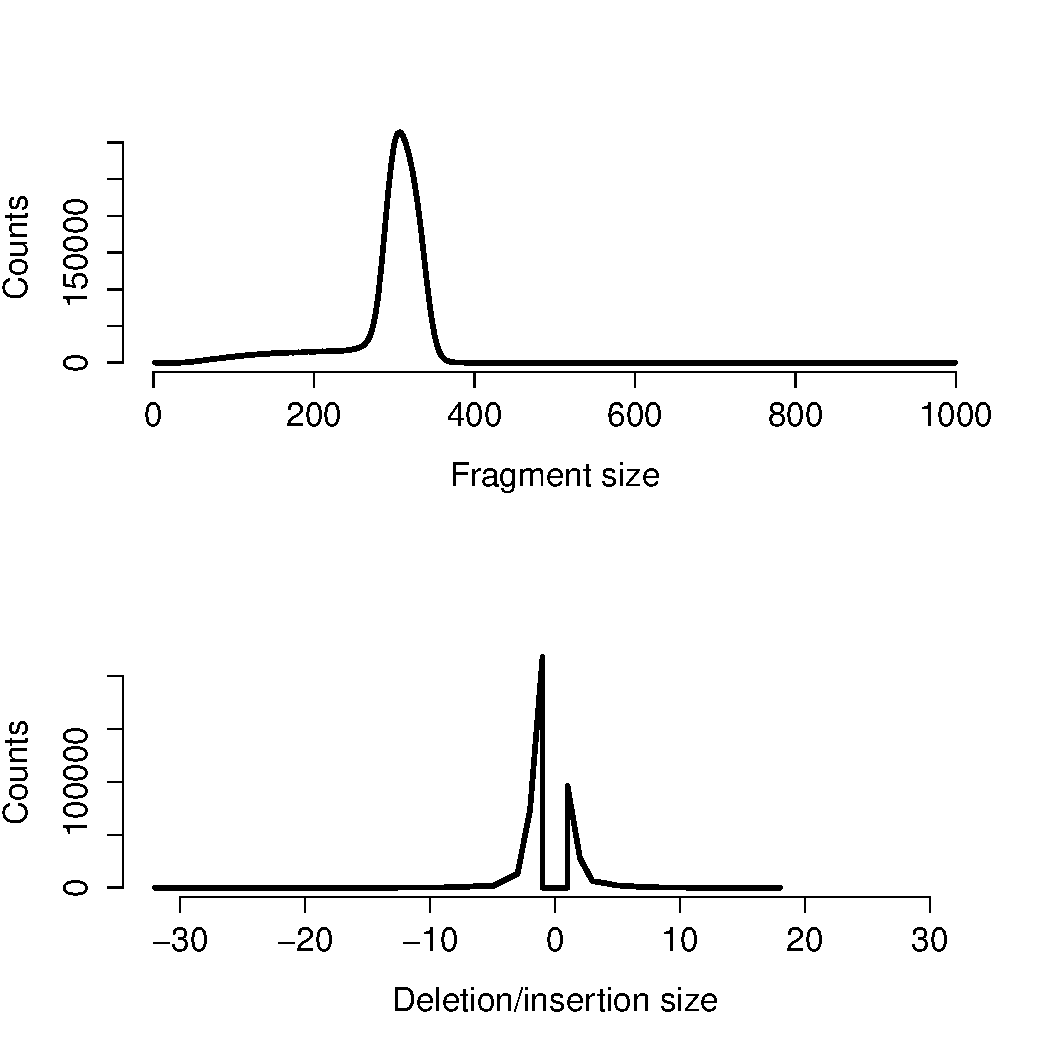
\includegraphics[width=\textwidth]{empDists-1}
  \caption{Top: empirical fragment size distribution for PG0051-C.  Bottom: empirical deletion (negative values) and insertion (positive values) length distribution for the same sample.}
  \label{fig:empDists-1}
\end{figure}

\subsubsection{Covariate table}

Finally, we construct the covariate table: a set of empirical distributions for various error events conditioned on the following:

\begin{enumerate}
    \item type (SNP, insertion, deletion)
    \item end of pair (first end or second end)
    \item strand (positive or negative)
    \item $5'$ dinucleotide context
    \item position in read
    \item first base of error sequence (empty for deletions)
\end{enumerate}

For each read, we increment an element in a table that corresponds to these six covariates.  The code to do so is contained in our \texttt{GenerateReadSimProfile} module.

\subsection{The read simulator}

With the coverage and read profiles in hand, we are finally ready to simulate reads.  We advance through each base of the simulated genome, reading the coverage profile as we traverse.  At each site, we use the coverage profile to dictate the number of fragments that must be generated and how many of those fragments should contain errors, thus modelling regions of the genome with higher or lower error rates.  We then generate fragments, sampling fragment lengths from the empirical fragment length distribution.  If a read is to contain an error, as specified by the coverage profile, we construct a read-specific error profile for mismatches, insertions, and deletions.  These profiles take into account the preceeding dinucleotide context for each position in the read\footnote{To handle the first and second positions in the read, which do not have a dinucleotide context, we simply extract a read by starting two nucleotides into the simulated fragment.}, the end of the pair being simulated, whether the fragment came from the positive or negative strand, and the first nucleotide of the error to be incorporated (not applicable for deletions).  

\begin{sidewaysfigure}[h!]
  \centering
    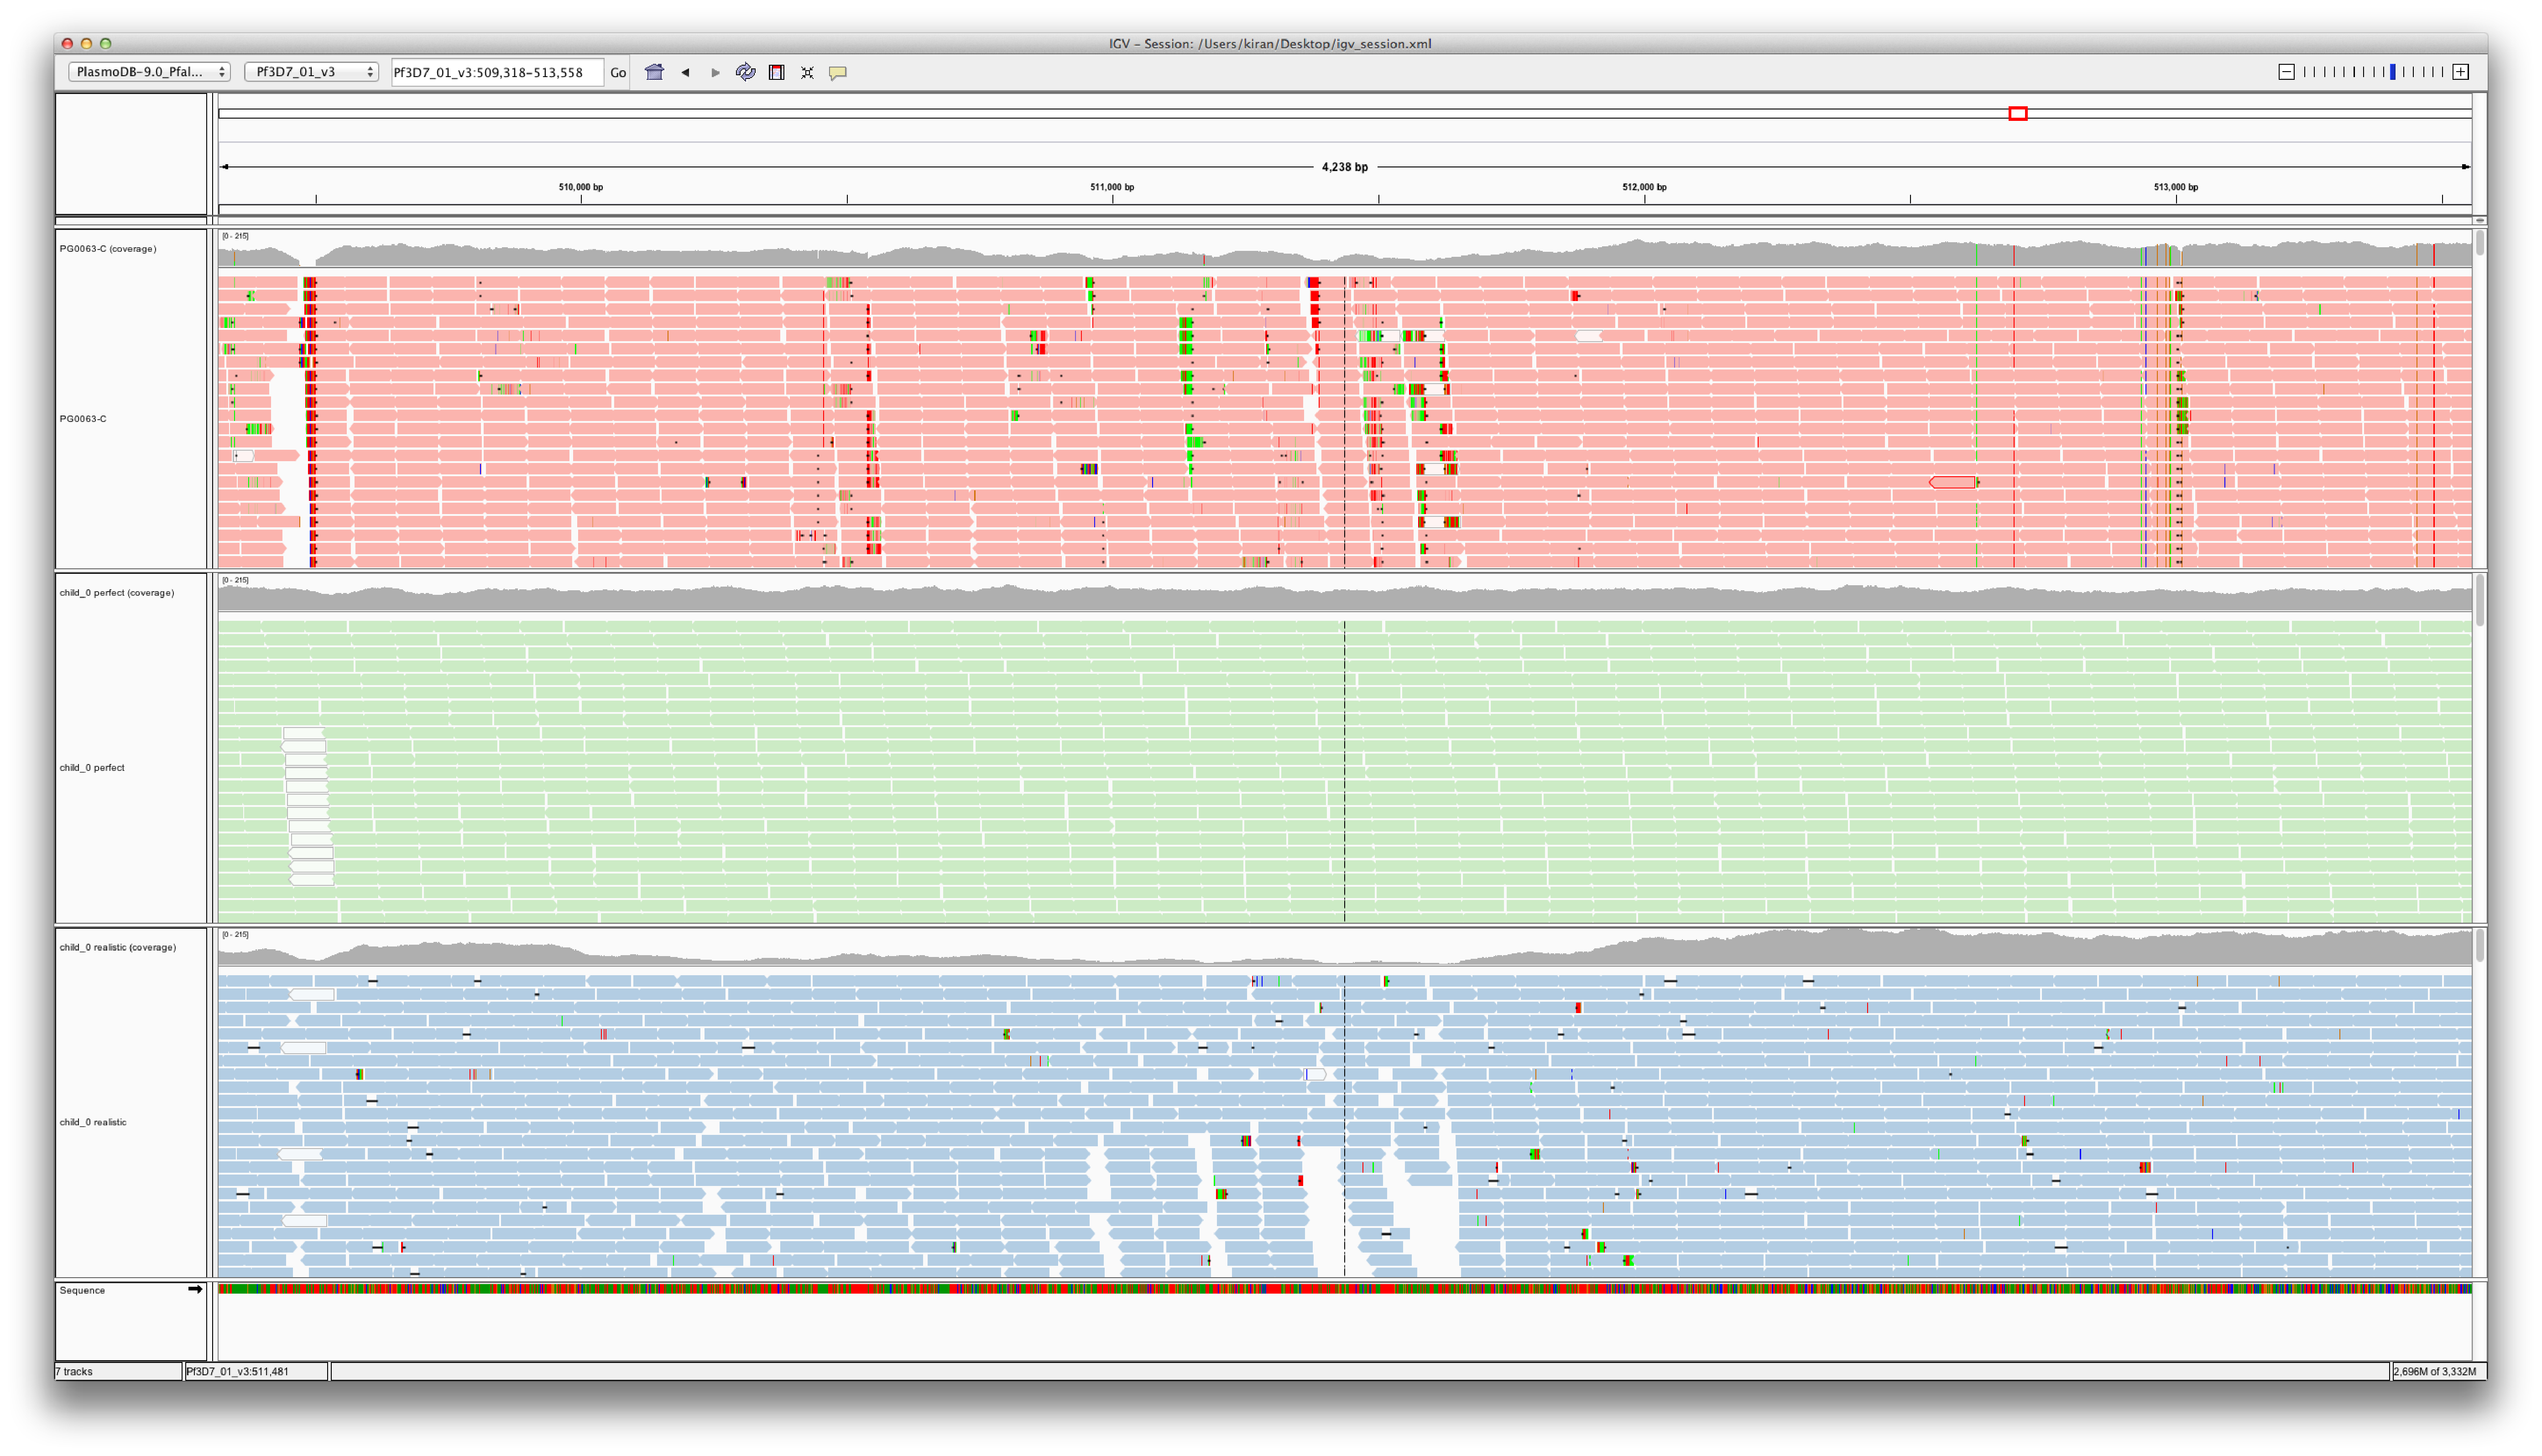
\includegraphics[width=\textwidth]{simreads}
  \caption{Read datasets for real (top panel), simulated perfect (middle panel), and simulated realistic (bottom panel) data.}
  \label{fig:simreads}
\end{sidewaysfigure}

\section{The simulated dataset}

With our genome and read simulation framework now complete, we simulated the genomes of $20$ progeny from a pseudo 3D7xHB3 cross.  The precise counts of variant types per sample are shown in Table \ref{tb:simstats}.  For each sample, we generated two datasets: a so-called "perfect" dataset (uniform coverage, perfect reads), and a so-called "realistic" dataset (non-uniform coverage, imperfect reads).  Both datasets contain approximately $150x$ coverage.

\begin{table}[]
\centering
\caption{\textit{De novo} variant counts for each of the $20$ simulated children.}
\label{tb:simstats}
\begin{tabular}{lrrrrrrrrrr}
\toprule
  & DEL & GC & INS & INV & NAHR & RECOMB & SNP & STR\_CON & STR\_EXP & TD\\
\midrule
0 & 22 & 25 & 22 & 22 & 2 & 10 & 5 & 3 & 3 & 26\\
1 & 21 & 21 & 21 & 21 & 2 & 10 & 23 & 11 & 11 & 26\\
2 & 11 & 22 & 11 & 11 & 2 & 8 & 13 & 22 & 22 & 8\\
3 & 25 & 17 & 25 & 25 & 2 & 32 & 23 & 17 & 17 & 21\\
4 & 4 & 23 & 4 & 4 & 2 & 8 & 14 & 16 & 16 & 12\\
5 & 26 & 23 & 26 & 26 & 2 & 37 & 28 & 5 & 5 & 8\\
6 & 13 & 17 & 13 & 13 & 2 & 15 & 27 & 23 & 23 & 4\\
7 & 1 & 22 & 1 & 1 & 2 & 30 & 28 & 5 & 5 & 12\\
8 & 26 & 16 & 26 & 26 & 2 & 16 & 16 & 13 & 13 & 8\\
9 & 4 & 23 & 4 & 4 & 2 & 25 & 23 & 23 & 23 & 21\\
10 & 12 & 20 & 12 & 12 & 2 & 16 & 23 & 19 & 19 & 27\\
11 & 13 & 19 & 13 & 13 & 2 & 7 & 20 & 18 & 18 & 17\\
12 & 19 & 20 & 19 & 19 & 2 & 8 & 14 & 5 & 5 & 28\\
13 & 10 & 20 & 10 & 10 & 2 & 25 & 13 & 28 & 28 & 11\\
14 & 28 & 18 & 28 & 28 & 2 & 8 & 3 & 29 & 29 & 17\\
15 & 27 & 22 & 27 & 27 & 2 & 30 & 5 & 19 & 19 & 2\\
16 & 23 & 22 & 23 & 23 & 2 & 12 & 29 & 24 & 24 & 17\\
17 & 17 & 22 & 17 & 17 & 1 & 10 & 28 & 13 & 13 & 11\\
18 & 23 & 18 & 23 & 23 & 2 & 8 & 1 & 21 & 21 & 18\\
19 & 22 & 22 & 22 & 22 & 2 & 17 & 19 & 3 & 3 & 2\\
\bottomrule
\end{tabular}
\end{table}

\section{Summary}

Unlike many other genome and read simulation software packages, our framework is able to generate realistic genomes and reads that exhibit allelic recombinations, non-allelic recombinations, a wide (and tuneable) spectrum of \textit{de novo} variants, and reads with realistic sequencing properties.  Rather than requiring a user to specify recombination rates, coverage levels, insert size distributions, and sequencing error rates (all of which may deviate wildly from real data), we have adopted the point of view that the end goal is to simulate data similar to a dataset one already possesses.  By drawing from empirical distributions derived from real data, we should find that the performance of our software on simulated data is informative of its capabilities on real data.

We do note a minor error in our simulation.  When producing empirical distributions for the lengths of indel errors, we treated insertions and deletions as separate events needing separate distributions.  However, inspecting these distributions more closely, we notice a bias: more deletion errors are present than insertion errors.  This is likely to be an artifact of read mapping, rather than of biology or even of sequencing.  Reads with insertions are typically more troublesome to place on a reference genome correctly than reads with deletions.  Still, it would have been more appropriate to sample insertion and deletion error lengths from the same distribution.  This error is not expected to compromise the results from the simulation.

We also note a deliberate omission: sample contamination.  Sample contamination by non-\textit{P. falciparum} data could generate false positive calls if, for instance, a child's sample is contaminated but the parents are not.  This point will be discussed in greater detail when examining validation data in Chapter \ref{cg:realdata}.
